\documentclass{article}
\usepackage[ngerman]{babel}
\usepackage[utf8]{inputenc}
\usepackage{graphicx} 
\usepackage{svg}
\graphicspath{{img/}}
\usepackage{geometry}
\geometry{a4paper, top=25mm, left=30mm, right=25mm, bottom=20mm}

\begin{document}

\section{Einführung}
Der Inhalt dieser Dokumentation besteht darin, die Umsetzung von eigenen SW-Treiber für eine Microcontroller-Plattform in Simulink zu erläutern. Hierfür wird zuerst die allgemeine Funktionsweise und insbesondere der Codegenerationsprozess mit Simulink diskutiert. Im Anschluss wird eine Übersicht über die verschiedenen Möglichkeiten dargestellt um eigene Simulink-Blöcke zu erstellen und in Quellcode zu übersetzen. MathoWorks sowohl Online- als auch PDF-Dokumentationen zur Verfügung, auf welche auch durchgehend verwiesen wird.

\newpage
\section{Funktionsweise von Simulink}
Simulink ist eine auf Blockschaltbildern basierende Programmierplattform, welche ursprünglich dazu gedacht war Differentialgleichungen numerisch zu lösen und Simulationen durchzuführen. Im Verlauf der Zeit wurde diese Basis kontinuierlich erweitert und unterstützt mittlerweile zahlreiche Funktionen. Eine bemerkenswerte Funktionalität von Simulink ist die Generation von Quellcode für Microcontroller. Damit können sowohl in kurzer Zeit umfangreiche Applikationen entworfen werden als auch durch Kommunikationsprotokolle zwischen Host- und Target-Plattform HiL-, SiL- und PiL-Simulationen durchgeführt werden. Somit stellt es ein mächtiges Werkzeug dar um Hardwarebausteine wie Sensoren und Microcontroller auszuwerten und daraufhin Filter und Regelungssysteme zu entwerfen.

In den folgenden Abschnitten werden die verschiedenen Ausführungsmodi und der Simulationsprozess von Simulink näher erklärt.

\subsection{Ablauf einer Simulink-Simulation}
Der Ablauf einer Simulation läuft in verschiedenen Phasen ab. Zuerst wird ein Model initialisiert. Hierbei werden die Datentypen, Weiten und Abtastraten der Blöcke und Signale festgelegt. Anschließend werden die Blockparameter ausgewertet und die Blockreihenfolge zur Ausführung bestimmt. Im nächsten Schritt wird die Simulation in einer Schleife ausgeführt. Das einmalige durchlaufen dieser Schleife wird auch als Simulationsschritt (Simulation step) bezeichnet. Der Aufbau der Simulationsschleife hängt von den Eigenschaften des Modelles ab. Besitzt ein Simulink-Modelle Blöcke mit variablen Abtastraten wird vor jedem Simulationsschritt dessen Ausführungszeitpunkt berechnet. Bei einem Modell fixen Abtastraten wird diese Berechnung nicht benötigt. Außerdem wird zwischen Blöcken mit diskreten und kontinuierlichen Zuständen unterschieden. Ein Block mit diskreten Zuständen wird einmal pro Simulationsschritt aufgerufen um seinen, für diesen Simulationsschritt, aktuellen Zustand und Ausgangswerte zu berechnen. Bei einem Block mit kontinuierlichen Zuständen wird dieser mit einer höheren Abtastrate als das restliche Model aufgerufen. In diesen Aufrufen werden die aktuellen Ausgangswerte und Ableitungen des Blocks berechnet.

\begin{figure}[h]
	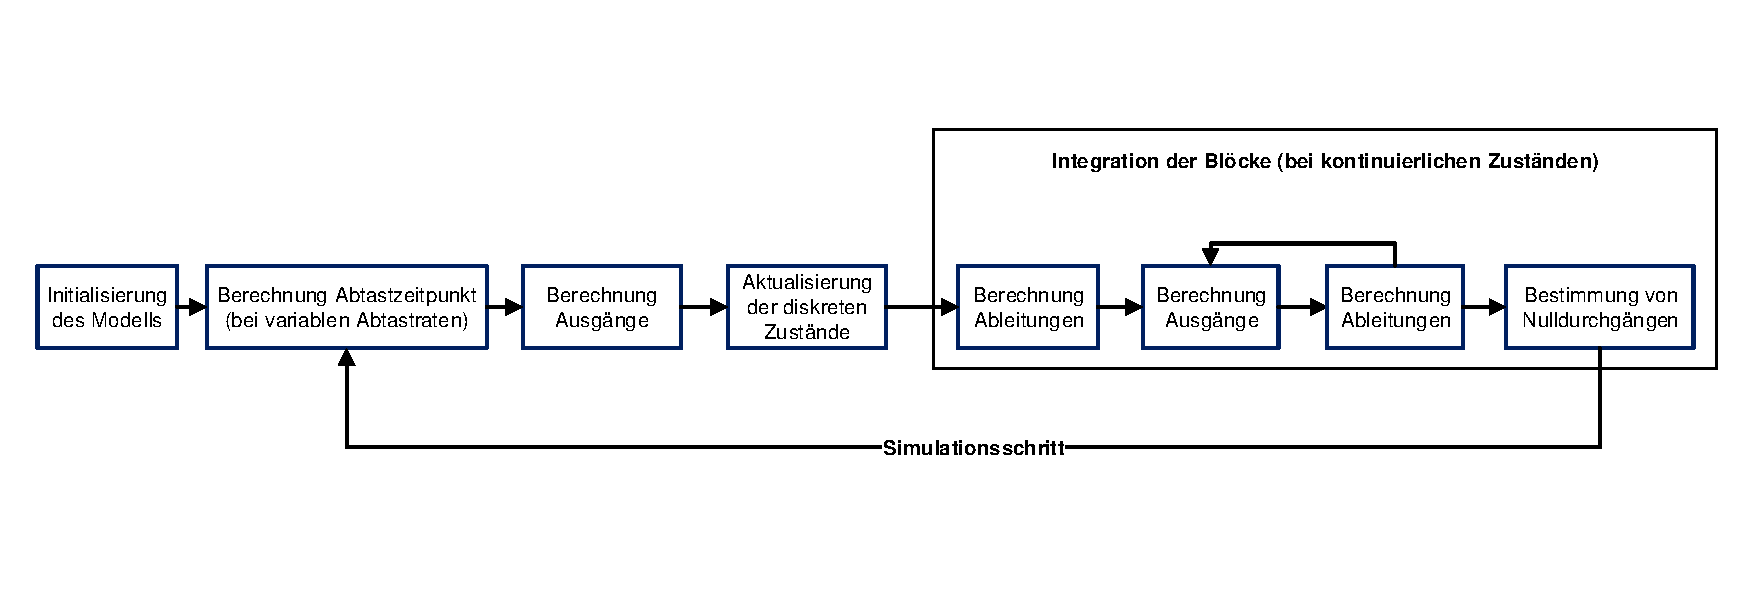
\includegraphics[width=\linewidth]{AblaufSimulation}
	\caption{Ablauf einer Simulation, Quelle: eigene Darstellung, Inhalt aus \cite{SFunc}}
\end{figure}

\subsection{Codegeneration mit Simulink}
Simulink bietet neben der Standardausführung eines Modell auch die Generation von Quellcode, der sowohl auf der Host- als auch auf anderen Zielplattformen ausgeführt werden. Die hierfür benötigten Produkte sind \textit{Simulink-Coder}\footnote{Früher als Real-Time-Workshop bekannt, deshalb wird in vielen Quellen nach wie vor von dem Real-Time-Workshop bzw. RTW gesprochen.} als Basis und ggf. \textit{Embedded-Coder}, welcher die Generation von optimierten C/C++-Code für Microcontroller-Plattformen ermöglicht. Die folgenden Abschnitte stellen den Ablauf einer Codegenration für Modelle mit einfachen, fixen Abtastraten vor. Für weitere Details über die Codegeneration von komplexen Modellen, welche beispielsweise variable Abtastraten, kontinuierliche Zustände und asynchrone Scheduling-Strategien verwenden, sei auf \cite{SimCoder} und \cite{EmbCoder}.

\subsection{Ablauf einer Simulink-Codegeneration}
Der Beginn einer Codegeneration ist identisch mit der üblichen Simulation. Das heißt, dass die Signale, Blockparameter und Abtastraten evaluiert werden. Anschließend legt Simulink die Ausführungsreihenfolge der Blöcke fest. Anschließend erstellt \textit{Simulink-Coder} eine RTW-Datei (.rtw), welche diese Informationen über das Modell enthält. Im nächsten Schritt wird die RTW-Datei dem \ac{TLC} übergeben, welcher die Generation des Quellcodes durchführt. \ac{TLC} ist eine von TheMathWorks entwickelte Programmiersprache bzw. der Interpreter, welche diese auswertet. Diese Programmiersprache ermöglicht einerseits die Auswertung von RTW-Dateien, andererseits können auch Code-Datein in beliebigen Sprachen erstellt werden. Für mehr Informationen über die Funktionsweise und Syntax von \ac{TLC} sei auf \cite{TLC} verwiesen.

Für die Codegeneration benötigt der \ac{TLC} neben der RTW-Datei des Modelles, ein \ac{STF}, ein \ac{TMF}, die Standard-TLC-Bibliothek und die \ac{TLC}-Dateien der einzelnen Blöcke, welche die Vorschrift für die Codegeneration des Blocks enthalten.

\begin{figure}[h]
	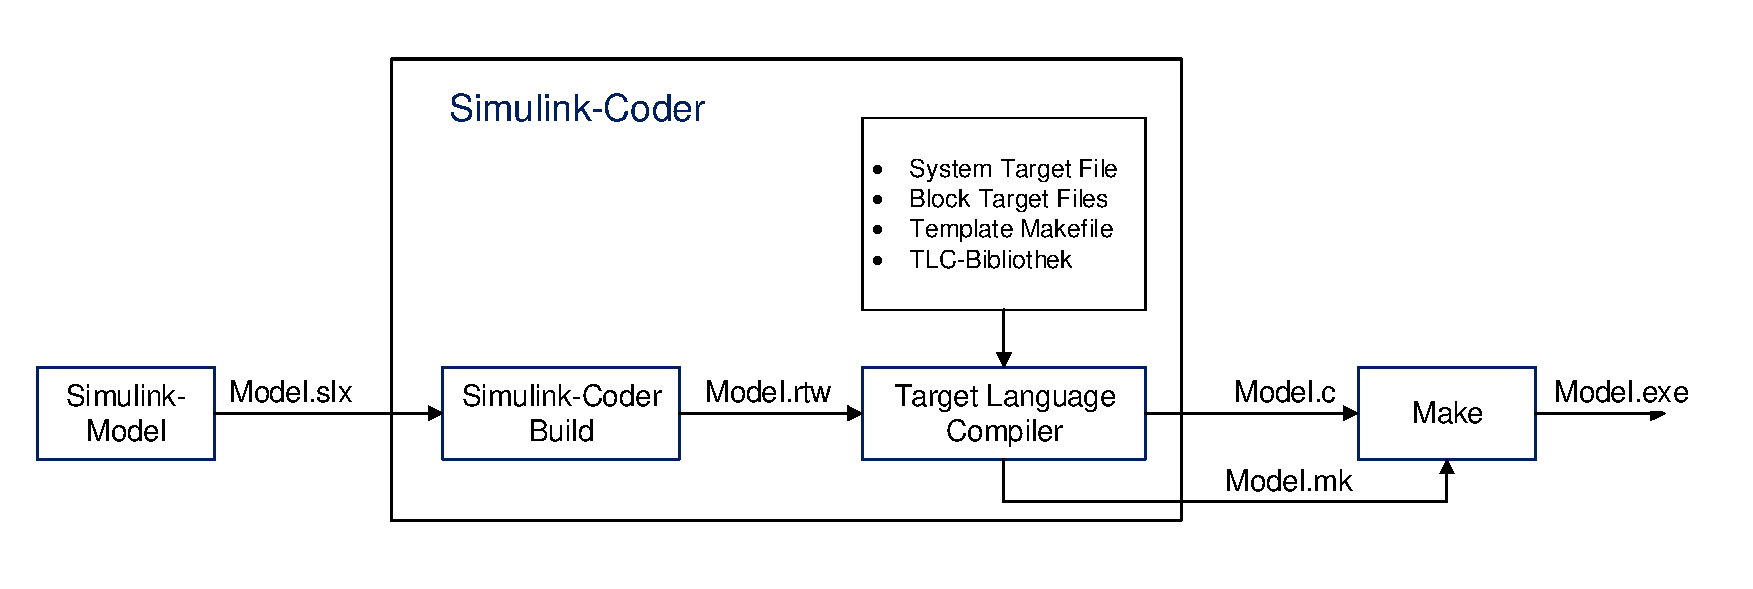
\includegraphics[width=\linewidth]{AblaufCodegeneration}
	\caption{Ablauf Codegeneration, Quelle: eigene Darstellung, Inhalt aus \cite{TLC}}
\end{figure}

\subsubsection{System Target File}
Das \ac{STF} stellt den Ausgangspunkt der \ac{TLC}-Codegeneration dar. In dieser Datei werden zuerst die Grundeinstellungen, wie z.B. das Codeformat und die Programmiersprache festgelegt. Anschließend werden eigenen Simulink-Blöcken TLC-Dateien zugeordnet, welche die Generationsvorschriften enthalten. Im nächsten Schritt wird die Ausführung der Simulink-Blöcke in entsprechender Reihenfolge in Quellcode übersetzt. Hierfür wird in der Regel die Datei "codegenentry.tlc" verwendet, welche von Simulink bereitgestellt wird. Diese Datei ordnet den Standard-Blöcken die entsprechenden TLC-Dateien zu, initialisiert globale Variablen und führt die Codegeneration eines einzelnen Simulationsschrittes durch. Zuletzt wird eine TLC-Datei inkludiert, welche eine main-Datei erstellt. In der main-Routine werden ggf. allgemeine Ressourcen initialisiert und die Simulationsschritte, den Abtastraten entsprechenden, aufgerufen.

\subsubsection{Template Make File}
Der \ac{TLC} erzeugt bei der Codegeneration ein Makefile um den Quellcode in ein ausführbares Format zu übersetzen. Das Makefile wird von einem \ac{TMF} abgeleitet, in welchem unter anderem die Toolchain, zusätzliche Bibliotheken und Compiler-Einstellungen festgelegt werden. Somit ermöglicht es ein \ac{TMF} auch Modelle auf beliebigen Zielplattform auszuführen, insofern eine Cross-Compiler-Toolchain zur Verfügung steht.

\newpage
\renewcommand\refname{Literaturverzeichnis}
\begin{thebibliography}{}
	\bibitem{SFunc} TheMathWorks, "Writing S-Functions", März 2016
\end{thebibliography}
\end{document}